\section{3G}

3G modulet testes som et selvstændigt modul. 
Testene der udføres er PUT og GET, da det er disse metoder der er implementeret på dronen. 
For at udføre tests med 3G modulet, kræves en fungerende server der tillader HTTP requests. For kun at have fokus på en enhed, anvendes projektets webserver ikke. Istedet er hjemmesiden requestb.in[X] anvendt, da requestb.in tillader HTTP kommunikation. Ved Requestb.in får man en URL, denne URL anvendes til både PUT og GET requests.

På figur \ref{fig:get_req} vises et GET request til en requestb.in server. I dette tilfælde: requestb.in/15zd1kn1. Den første linje efter \textit{data:} fortæller om requestet er gennemført succesfuldt eller om der er sket en fejl. Svaret 200 ok betyder at requestet er gået igennem og det ønskede data er hentet. 

\begin{figure}[H]
\centering
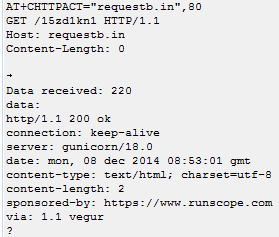
\includegraphics[width=0.4\textwidth]{Billeder/Test/get_requestbin.png}
\caption{GET Request}
\label{fig:get_req}
\end{figure}

På figur \ref{fig:put_req} vises PUT requesten til requestb.in. RAW BODY viser det data der er sendt og HEADERS indeholder en information med besked statussen.

\begin{figure}[H]
\centering
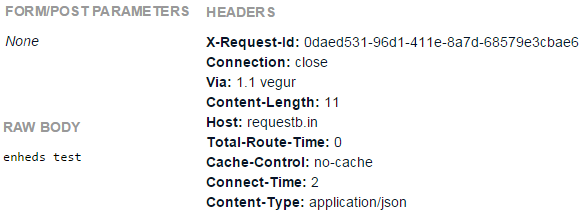
\includegraphics[width=0.8\textwidth]{Billeder/Test/put_request.png}
\caption{GET Request}
\label{fig:put_req}
\end{figure}
